\chapter{Related Work} 
\label{chap:relatedwork}

In this chapter we describe platforms, systems and approaches developed by others which are relevant for the Healthbank system. First we focus on existing health systems and compare them to Healthbank. In the second part of this chapter we describe some social networks and compare the way they set up connections among users and how they share data with our approach.


%%% ------------- SECTION -------------
\section{Health Systems}

There have been many different approaches to build a health platform such as the one we plan for Healthbank.  \newline
In the United States of America the standardisation of health data started out with the concept of XML bound data. This XML data can be carried around or saved at a save place by patients themselves and shared via email. This standard is called the Continuity of Care Record (CCR)~\cite{kibbe2004continuity}. Even though this was a good start and patients were in possession of parts of their health data, XML is not particularly a user friendly data format. \newline
In 2008 Google started its service Google Health which implemented the CCR standard. The system allowed their users to create a centralized health profile. Data was integrated either by hand by the users themselves or by accounts on partnered health service providers. Google partnered with about thirteen organizations in total~\cite{googlehealthwiki}. The service was free to use and did not contain any advertisement. Google retired the system on January 1, 2012 officially~\cite{googleblog} because of the fact that it 
\begin{quote}
"did not catch on the way we would have hoped, but did serve as influential models."
\end{quote} 
Therefore many of the official system and API information is not accessible anymore on the Google website. A short introduction to the system is e.g. provided by \emph{The Health IT Synthesis Project blog~\cite{hisp}} though. From the fact that Google found some great partners we are very positive that external providers can be found to create applications and visualizations for the Healthbank system too. Another thing we can learn about Google Health is that people are understandably very sensitive with their health data. Trust in a platform is a big concern. Hence, we think that it would be best if Healthbank will become a non-profit organization. 

Apart from Google, there is also a system by Microsoft called HealthVault~\cite{healthvault}. According to Wikipedia this service is running since October 2007 in the USA and since June 2010 in the UK as well. Users first have to create an account and can then store health information such as medications, blood pressure values, allergies, fitness level, x-rays, lab results, health history as well as conditions and illnesses. With the system users can also set and print emergency information. Thanks to the introduction of Windows 8, Microsoft made HealthVault available for mobile devices such as smartphones or tablets. The system allows sharing of data with others. There are about 15 applications and more than 150 devices, which can integrate with HealthVault to read and store data. These are external applications such as e.g. an iPhone application which can send data to HealthVault or receive data for motivation and analysis purposes. Devices include e.g. smart scales and GPS watches for running. This system is up and running for almost five years now and still has not become a huge success. Compared to the system by Microsoft which uses mostly structured data, Healthbank will accept almost all kind of data. The integration of applications and devices shall also be an important part of the Healthbank system.

Next to the commercial systems there are also some open-source projects worth mentioning. For example there is a project called Open mHealth~\cite{openmhealth} which is according to their website
\begin{quote}
"an open architecture to enable improved integration among mobile health solutions, to unlock the full potential for mHealth. Through a shared set of open APIs\textsuperscript{\ref{API}}, open and proprietary software modules, applications and data can be `mixed and matched`, and more meaningful insights derived through reusable data processing and visualization modules."
\end{quote}
We especially like the approach to integrate mobile applications and wearable devices and how they combine these values. We try to build on top of this by the integration of external applications. These shall allow to add the data of mobile applications and devices to the user account on our system.

Another interesting open-source project is Indivo~\cite{indivohealth}~\cite{adida2010indivo}~\cite{mandl2007indivo}. The project is supported by the MIT, the Harvard Medical School and the Boston Children's Hospital Informatics Program. On the Indivo website they describe their project like this: 
\begin{quote}
"Indivo is the original personal health platform, enabling an individual to own and manage a complete, secure, digital copy of her health and wellness information. Indivo integrates health information across sites of care and over time. Indivo is free and open-source, uses open, unencumbered standards, including those from the SMART Platforms project~\cite{smart} and is actively deployed in diverse settings."
\end{quote}
By having a look into their documentation~\cite{indivoDoc} we find that the system is written in Python, communication is done via HTTPS and authentication using OAuth. Their backend server - the Indivo X server - deals with accounts and records as well as with authentication and authorization. The system further provides a GUI for administrators and user applications. On top of that they provide a web based GUI - the Indivo User Interface or Indivo Chrome. The system allows users to add user applications which have a web interface embedded in an iframe (allows to places another HTML document in the frame). Also there are admin applications which are able to connect to the X server and create new accounts, change them, as well as change ownership and metadata of records. But they are not allowed to access the content of records. Figure \ref{fig:indivoArch} illustrates Indivo`s basic architecture.

% Figure 2.1
\begin{figure}[ht]
%\centering
%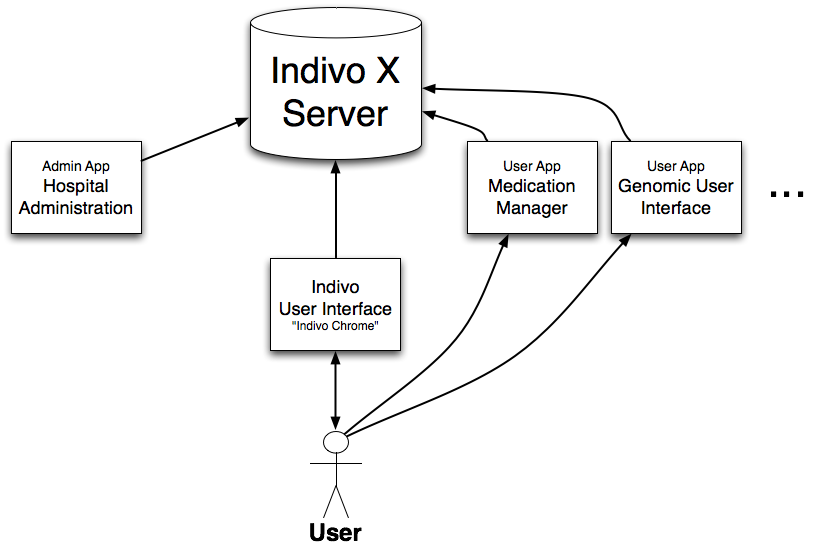
\includegraphics[width=408px,height=274px]{indivo-arch.png}
\makebox[\textwidth][c]{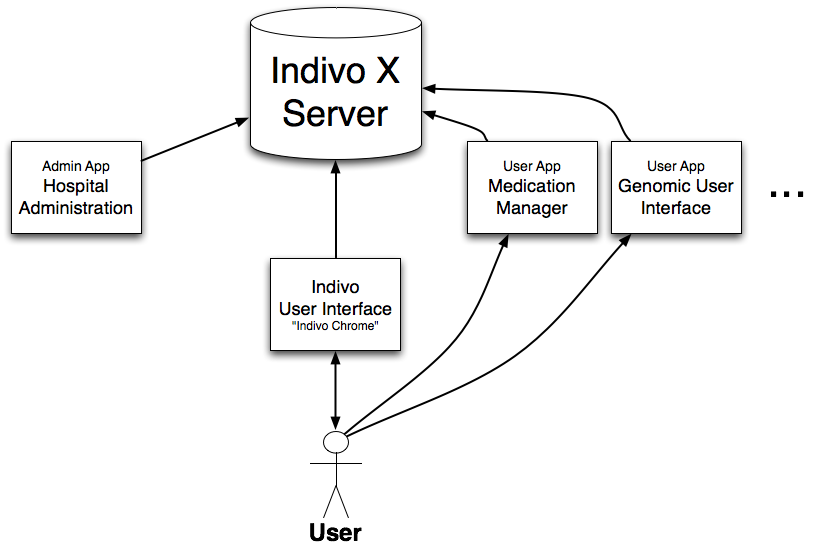
\includegraphics[width=408px,height=274px]{indivo-arch.png}}%
\caption{Indivo architecture overview.~\cite{indivoDoc}}
\label{fig:indivoArch}
\end{figure} 

A record in Indivo consists of a single or multiple documents and can be accessed by one or multiple accounts. Nevertheless there is one account defined as the owner of the record. There are different data models based on Django`s object-relational mapping (ORM)~\cite{django}. A query API\textsuperscript{\ref{API}} and a reporting API make these data models queryable. Indivo provides a SDMX\footnote{Wikipedia: Statistical Data and Metadata eXchange (SDMX) is an initiative to foster standards for the exchange of statistical information.} schema to define the format of incoming data in their SDMX specification language. The more XSD schemas (schema for XML) are used for XML validation. The pipeline for incoming data is illustrated in figure \ref{fig:indivoPipeline}. As mentioned before this data has to be in XML format and has to agree to a XSD schema. Then it is transformed according to a transform output format and converted into one or more fact objects for storage. Via the reporting API one can then query the database for matching facts. These facts will be serialized to XML or JSON for the app to retrieve.

% Figure 2.2
\begin{figure}[ht]
%\centering
%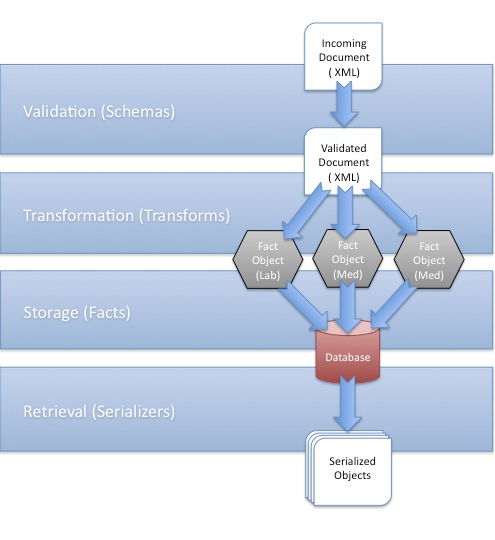
\includegraphics[width=330px,height=360px]{indivo-data-pipeline.png}
\makebox[\textwidth][c]{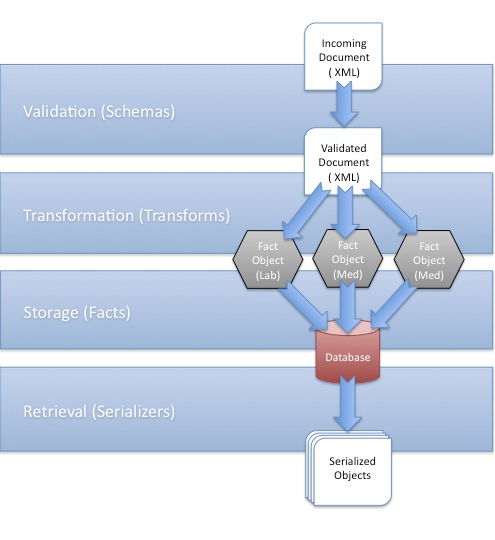
\includegraphics[width=330px,height=360px]{indivo-data-pipeline.png}}%
\caption{The Indivo data pipeline visualized.~\cite{indivoDoc}}
\label{fig:indivoPipeline}
\end{figure} 

A fact is a single data point, e.g. one medication, formatted according to a data model (here e.g. the medication data model). Indivo provides a messaging and notification system similar to emails. Messages have a subject and a body. They can be sent to records as well where they will be rerouted to the owner and all accounts that have full access to that record. To register an application with Indivo, an application manifest is needed. The SMART Project`s syntax is used for this with some Indivo-specific parameters. In the manifest the application can define among others the Indivo version to use, whether it can be used in an iframe or not, if it has an UI and the OAuth callback URL. The more there are the usual information such as name, description, version, icon, etc. The Indivo project contains many interesting ideas and approaches which we used as a starting point for our discussion on the architecture of Healthbank. In contrast to Indivo we decided not to use schemas and force others to our way of dealing with record entries. This allows to store any kind of structured and unstructured data and needs less integration work for application providers. On the contrary, this leads to less control by us. Asking queries on the data set gets more difficult. On the other hand we do not give applications that much control. E.g. an admin application in Indivo can create new accounts and change ownership of records. All applications are allowed to do on the Healthbank system is adding new entries to a user and illustrate them. So applications will not interfere with our goal of giving the users full control of their health data.

There are other interesting platforms on the web such as e.g. 23andMe~\cite{23andme}, which provides rapid genetic testing and a lot of information about a user`s DNA. On PatientsLikeMe~\cite{plm}\label{patientslikeme} patients with similar diseases can interact and share experiences with each other. From these two platforms we can learn that it is very important for users to get information and to get into contact with people who suffer from similar diseases. Therefore Healthbank shall introduce a health knowledge platform that allows users to quickly find information about diseases and medications. With the help of a clever search engine the doctors and individual people shall also be able to search for similar patients.

%%% ------------- SECTION -------------
\section{Social Platforms}
According to the Oxford Dictionaries a social network is 
\begin{quote}
"a network of social interactions and personal relationships"
\end{quote}
Therefore Healthbank will, to a certain extent, be a social network as well. Its focus is clearly to have a centralized form of storing the user`s health data. But the system will also allow to share data with doctors, hospitals as well as with friends and family. . Furthermore it allows to communicate via a messaging system and has the ability to integrate external applications. Because of these facts, we will now have a look at two of the biggest among the variety of social networks that exist today, which are Facebook~\cite{facebook} and Google+~\cite{googlePlus}.

The Google+ Wikipedia entry tells us that it was launched by the Google Inc. in 2011. By now it has more than 500 million registered users out of which about half of them are active users (they log in at least once a month). With Google+, Google integrated several services such as their image organizer and sharing service Picasa or their messaging service Google Talk (which is now replaced by Hangouts). Also it integrates rather well with other Google services such as YouTube, Gmail, Calendar or Drive.\newline 
The part we are mainly interested is the way Google+ deals with connections between users. Google+ organizes other people related to the current user in so called \emph{circles}. A user can add other users to one or multiple of his circles. A circle is somewhat like a group for sharing. Every post, photo, event, etc. can be shared with these circles. This way the user has a very fine-grained control over sharing. In contrast to other social networks, who usually operate with a one-to-one friend relation, these circle relations are only one-directional. In other words user $A$ can have user $B$ in one of his circles, but $B$ does not need to have $A$ in any of his circles. This fact is used e.g. with the so called 'Following' circle which allows users - similar to Twitter - to follow other people they do not know, but whose posts they find interesting (e.g. celebrities). We do like this circle management and took it as a starting point for our prototype user management and sharing system.

Facebook is the world`s biggest social network founded by Mark Zuckerberg in 2004. Today it has more than a billion users around the globe. More than 600 million users access Facebook via a mobile device (Source: Wikipedia). Users have their own profile and can share posts, photos, videos or links with their friends. Others can comment and \emph{like} (an appreciation of content) these items. Users can interact with each other via a messaging as well as a chat system. Connections between users are bidirectional this means that for two users to be friends, both have to agree. \newline
With the Facebook App-Centre users get a variety of games, quizzes and other applications. These games and applications are either directly integrated in the Facebook look and feel or use the Facebook API to log into and get data from Facebook (e.g. developers can use Facebook for their page user management). These games allowed companies like Zynga to make a real fortune. Applications are allowed to add new posts to the user`s chronicle in the name of the user such as e.g. sharing a new high score in a game. We are particularly interested in the application integration since we plan to allow third-party providers to write applications for Healthbank as well. \newline
With their new Graph Search, Facebook is currently deploying, they allow to ask full text queries such as "people who like to mountain bike and live in my hometown" or "towns my family visited". We are planning to have a similar kind of search engine for researchers and doctors in order to answer questions like "people with high blood pressure living in Washington DC" or "people with similar symptoms like me".